% arara: xelatex: {shell: yes}
% %arara: biber
% %arara: xelatex: {shell: yes}
% %arara: xelatex: {shell: yes}

\documentclass[12pt]{article}

\usepackage{pst-knot} % не работает?

\usepackage{hyperref} % гиперссылки

\usepackage{tikz} % картинки в tikz
\usetikzlibrary{arrows.meta} % tikz-прибамбас для рисовки стрелочек подлиннее

\usepackage{microtype} % свешивание пунктуации

\usepackage{array} % для столбцов фиксированной ширины

\usepackage{indentfirst} % отступ в первом параграфе

\usepackage{sectsty} % для центрирования названий частей
\allsectionsfont{\centering}

\usepackage{amsmath} % куча стандартных математических плюшек
\usepackage{amssymb} % символы
\usepackage{amsthm} % теоремки

\usepackage{comment} % добавление длинных комментариев

\usepackage[top=2cm, left=1.2cm, right=1.2cm, bottom=2cm]{geometry} % размер текста на странице

\usepackage{lastpage} % чтобы узнать номер последней страницы

\usepackage{enumitem} % дополнительные плюшки для списков
%  например \begin{enumerate}[resume] позволяет продолжить нумерацию в новом списке

\usepackage{caption} % что-то делает с подписями рисунков :)

\usepackage{qcircuit} % для рисовки квантовых диаграмм
\usepackage{physics} % бракеты

\usepackage{answers} % разделение условий и ответов в упражнениях



\usepackage{fancyhdr} % весёлые колонтитулы
\pagestyle{fancy}
\lhead{Я завязал}
\chead{}
\rhead{КЛШ-2023 (46 сезон)}
\lfoot{}
\cfoot{}
\rfoot{\thepage/\pageref{LastPage}}
\renewcommand{\headrulewidth}{0.4pt}
\renewcommand{\footrulewidth}{0.4pt}



\usepackage{todonotes} % для вставки в документ заметок о том, что осталось сделать
% \todo{Здесь надо коэффициенты исправить}
% \missingfigure{Здесь будет Последний день Помпеи}
% \listoftodos — печатает все поставленные \todo'шки



\usepackage{booktabs} % красивые таблицы
% заповеди из докупентации:
% 1. Не используйте вертикальные линии
% 2. Не используйте двойные линии
% 3. Единицы измерения - в шапку таблицы
% 4. Не сокращайте .1 вместо 0.1
% 5. Повторяющееся значение повторяйте, а не говорите "то же"



\usepackage{fontspec} % что-то про шрифты?
\usepackage{polyglossia} % русификация xelatex

\setmainlanguage{russian}
\setotherlanguages{english}

% download "Linux Libertine" fonts:
% http://www.linuxlibertine.org/index.php?id=91&L=1
\setmainfont{Linux Libertine O} % or Helvetica, Arial, Cambria
% why do we need \newfontfamily:
% http://tex.stackexchange.com/questions/91507/
\newfontfamily{\cyrillicfonttt}{Linux Libertine O}

\AddEnumerateCounter{\asbuk}{\russian@alph}{щ} % для списков с русскими буквами
\setlist[enumerate, 2]{label=\asbuk*),ref=\asbuk*}

%% эконометрические сокращения
\DeclareMathOperator{\Cov}{Cov}
\DeclareMathOperator{\Arg}{Arg}
\DeclareMathOperator{\Corr}{Corr}
\DeclareMathOperator{\Var}{Var}
\DeclareMathOperator{\E}{\mathbb{E}}
\DeclareMathOperator{\lk}{lk}
\newcommand \hVar{\widehat{\Var}}
\newcommand \hCorr{\widehat{\Corr}}
\newcommand \hCov{\widehat{\Cov}}
\newcommand \cN{\mathcal{N}}
\let\P\relax
\DeclareMathOperator{\P}{\mathbb{P}}

\usepackage{multicol}

\usepackage[bibencoding = auto,
backend = biber,
sorting = none,
style=alphabetic]{biblatex}

\addbibresource{forecast_everything.bib}



% делаем короче интервал в списках
\setlength{\itemsep}{0pt}
\setlength{\parskip}{0pt}
\setlength{\parsep}{0pt}




\Newassociation{sol}{solution}{solution_file}
% sol --- имя окружения внутри задач
% solution --- имя окружения внутри solution_file
% solution_file --- имя файла в который будет идти запись решений
% можно изменить далее по ходу
\Opensolutionfile{solution_file}[all_solutions]
% в квадратных скобках фактическое имя файла

% магия для автоматических гиперссылок задача-решение
\newlist{myenum}{enumerate}{3}
% \newcounter{problem}[chapter] % нумерация задач внутри глав
\newcounter{problem}[section]

\newenvironment{problem}%
{%
\refstepcounter{problem}%
%  hyperlink to solution
     \hypertarget{problem:{\thesection.\theproblem}}{} % нумерация внутри глав
     % \hypertarget{problem:{\theproblem}}{}
     \Writetofile{solution_file}{\protect\hypertarget{soln:\thesection.\theproblem}{}}
     %\Writetofile{solution_file}{\protect\hypertarget{soln:\theproblem}{}}
     \begin{myenum}[label=\bfseries\protect\hyperlink{soln:\thesection.\theproblem}{\thesection.\theproblem},ref=\thesection.\theproblem]
     % \begin{myenum}[label=\bfseries\protect\hyperlink{soln:\theproblem}{\theproblem},ref=\theproblem]
     \item%
    }%
    {%
    \end{myenum}}
% для гиперссылок обратно надо переопределять окружение
% это происходит непосредственно перед подключением файла с решениями



\theoremstyle{definition}
\newtheorem{definition}{Определение}



\begin{document}

\tableofcontents{}

\section*{Анонс}
...

\newpage
\setcounter{section}{0}

\section{Встреча раз}


Узел: верёвка, соединяющая две стены \textit{или} замкнутая кривая в пространстве. 

Вяжем прямой или встречный узел. 

Упражнение. Завяжи произвольный узел и нарисуй его плоскую диаграмму. 

Упражнение. Занумеруй пересечения и запиши узёл, произжая по нему на машини и отмечая, 
сверху или снизу едешь по мосту, направо или налево ведёт поперечная дорога. 

А = Above, B = Below, L = Left, R = Right, AL = Above Left и так далее.

Упражнение. Нарисуй плоскую диаграмму по записи узла. 

Определение косы. 

\section{Встреча два}

Упражнение. Нарисуй плоскую диаграмму по записи. 

Три нити. Коса $b_1$. Коса $b_2$. Умножение кос. 

\newcommand{\daytwo}{
\begin{enumerate}
\item  \textit{Единичная} коса $1$ при умножении на любую косу не меняет её.

Как выглядит единичная коса на пяти нитях?
\item Коса $b_1^{-1}$ при умножении на косу $b_1$ должна порождать единичную косу.

Нарисуй косу $b_1^{-1}$ на трёх нитях.
\item Нарисуй косу $b_1 b_2 b_3^3 b_1^{-1} b_2 b_3^{-1}$ на четырёх нитях.
\item Правда ли, что $b_1 b_2 = b_2 b_1$? Правда ли, что $b_2 b_4 = b_4 b_2$?
\item Правда ли, что $b_1 b_2 b_3 = b_3 b_2 b_1$? Правда ли, что $b_2 b_1 b_2 = b_1 b_2 b_1$?
\item Нарисуй косу $b_1^3 b_2$ на трёх нитях, замкни её и запиши плоскую диаграмму полученного узла.
\item Перед тобой узлы:



Для каждого узла нарисуй косу, которая его порождает при замыкании. 
Запиши полученную косу.
\item Сколько узлов получается при замыкании косы $b_1^2 b_3^4$ на четырёх нитях?
\item Сколько узлов получается при замыкании косы $b_1 b_2^2 b_3^3 b_4^4 b_5^5$ на шести нитях?
\item Нарисуй узел $(AL)_1 (BL)_2 (AR)_3 (BR)_1 (AL)_4 (BL)_3 (AR)_2 (BR)_4$.
Нарисуй косу, которая при замыкании даёт этот узел. Запиши эту косу. 
\end{enumerate}
}

\newpage
\daytwo
\vfill
\daytwo

\newpage

Воровской узел. 


\newcommand{\dayfour}{
  \begin{enumerate}
    \item Какой узел $O$ при сложении с любым другим узлом $K$ не изменяет его, $K \# O = O \# K = K$? 
    \item Правда ли, что для узлов $K_1 \# K_2 = K_2 \# K_1$?
    
    \item Зацепи $n$ тривиальных узлов самым простым образом так, 
    чтобы при разрезании одного любого кольца всё зацепления распадалось на отдельные кусочки:

    \begin{minipage}{\linewidth}
      \begin{multicols}{3}
        \begin{enumerate}    
        \item Зацепление Хопфа, $n=2$;
        \item Зацепление Борромео, $n=3$;
        \item $n=4$;
      \end{enumerate}
    \end{multicols}
    \end{minipage}

    \item Используя движения Рейдемейстера перевиди одну картинку в другую
    
    \begin{minipage}{\linewidth}
      \begin{multicols}{2}
        \begin{enumerate}    
        \item 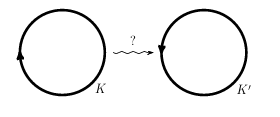
\includegraphics[scale=0.8]{pictures/trivial2trivial.png}
        \item 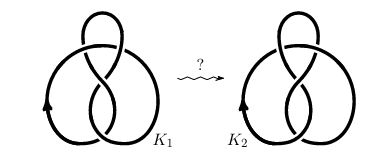
\includegraphics[scale=0.6]{pictures/eight2eight.png}
      \end{enumerate}
    \end{multicols}
    \end{minipage}
    
    
    \item Зарисуй движение Рейдемейстера $\Omega_1$ на диаграмме Гаусса и 
    запиши его в коде узла Гаусса. 

    Рассмотри все варианты.
    \item Как может выглядеть движение Рейдемейстера $\Omega_2$ на диаграмме Гаусса и 
    в коде узла Гаусса? 
    \item Как может выглядеть движение Рейдемейстера $\Omega_3$ на диаграмме Гаусса и 
    в коде узла Гаусса?
  \end{enumerate}
}

\newpage
\dayfour
\vfill
\dayfour
\newpage



\newcommand{\daysix}{
Для зацепления из двух компонент \textit{коэффициент зацепления} $\lk = (N_R - N_L) /2$, где $N_R$ — число мостов, 
где первая компонента проходит над второй и под мостом поток приходит с правой стороны, 
а $N_L$ — число мостов, где первая компонента проходит над второй и под мостом поток приходит с левой стороны.

Плоская диаграмма узла называется \textit{раскрашиваемой в три цвета}, если каждый отрезок узла от прохода под мостом до прохода под мостом 
можно раскрасить в один из трёх цветов так, чтобы в каждом пересечении встречались три цвета или один цвет.

\begin{enumerate}
  \item Какие из диаграмм можно раскрасить в три цвета по правилам?
  \item Для каждого двухкомпонентного зацепления посчитай коэффициент зацепления.
  \item Что происходит с коэффициентом зацепления, если первую компоненту считать второй, а вторую — первой?
  \item Что происходит с коэффициентом зацепления, если поменять направление обхода первой компоненты?
  \item Докажи, что движения Рейдемейстера сохраняют раскрашиваемость в три цвета.
  \item Докажи, что движения Рейдемейстера сохраняют коэффициент зацепления.
\end{enumerate}

}

\newpage
\daysix
\vfill
\daysix
\newpage

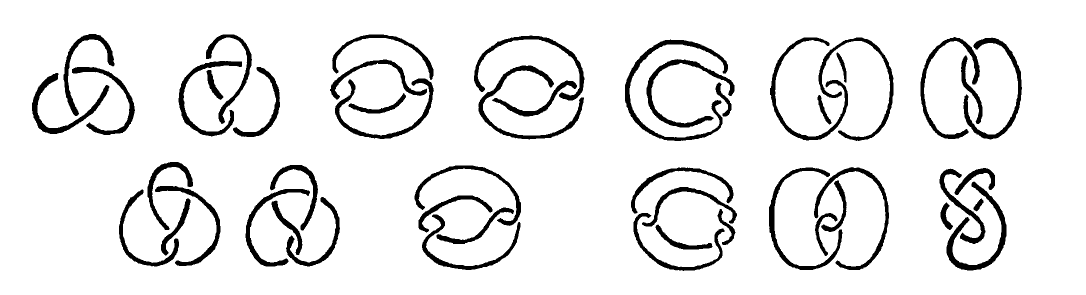
\includegraphics[scale=0.7]{pictures/two-lines.png}

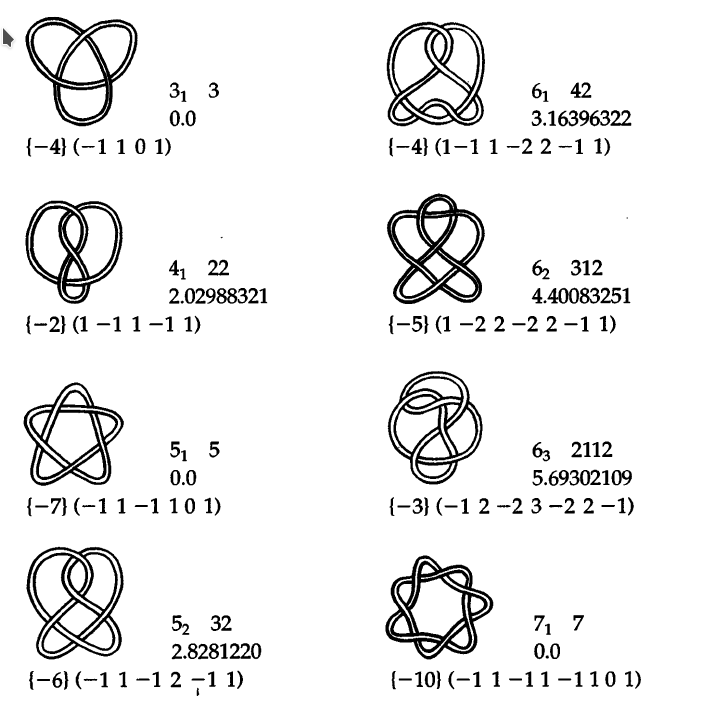
\includegraphics[scale=0.8]{pictures/small-knots.png}

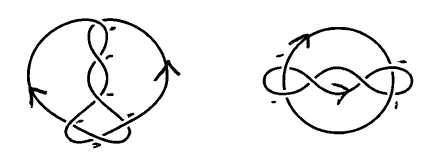
\includegraphics[scale=0.8]{pictures/linking-number-1.png}
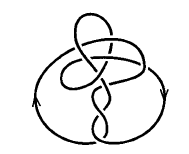
\includegraphics[scale=0.8]{pictures/linking-number-2.png}
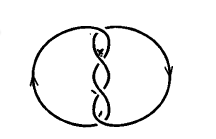
\includegraphics[scale=0.8]{pictures/linking-number-3.png}
\newpage

\section{Лог. КЛШ-2023}

Курс выбрали 7 школьников.

\begin{enumerate}
  \item 
\end{enumerate}

В теховском файле \verb|\newpage| стоит, чтобы легко было скопировать секцию, для печати двух копий подряд на одном листе.
Это позволяет экономить бумагу и время при печати :)

\subsection{Плакат}





\Closesolutionfile{solution_file}

% для гиперссылок на условия
% http://tex.stackexchange.com/questions/45415
\renewenvironment{solution}[1]{%
         % add some glue
         \vskip .5cm plus 2cm minus 0.1cm%
         {\bfseries \hyperlink{problem:#1}{#1.}}%
}%
{%
}%



\section{Решения}
\input{all_solutions}


\section{Источники мудрости}

\todo[inline]{передалать потом в bib-файл}

\begin{enumerate}
\item \url{https://ctan.org/pkg/braids}: рисование кос
\item \url{https://tex.stackexchange.com/questions/559167/}: шрифт с набором реалистичных узлов
\item \url{https://ctan.org/pkg/pst-knot}: десяток готовых узлов: не работает?
\item \url{https://ctan.org/pkg/spath3}: рисуем произвольные узлы
\item \url{https://ncatlab.org/nlab/show/SVG+images}: немного svg-картинок узлов, движения Рейдемейстера
\end{enumerate}

\printbibliography[heading=none]


\end{document}
